\section{Renormalization Group, Part III}

\subsection{Review - Effective Actions in Various Dimensions, Symmetries}
We've been recasting the Ising problem into a field theory. We dispensed of the short wavelength degrees of freedom - not by doing a hard integral but by manipulating the effective action. We saw the payoff which is that the form of the problem simplifies greatly when we look at the second transformation of the renormalization group.

For $D > 4$, we have:
\begin{equation}
    S_{\text{eff}}[\phi] = \int d^Dx \left(\frac{1}{2}(\nabla \phi(x))^2 + \frac{\tau}{2}\phi^2(x)\right)
\end{equation}
which starts to look very simple (only quadratic operators are marginal); we know how to solve theories for which the energy functional is just a Gaussian.

For $D = 4$, another operator becomes marginal, and for $D < 4$ it becomes relevant; i.e. we get a $\phi^4$ term:
\begin{equation}
    S_{\text{eff}}[\phi] = \int d^Dx \left(\frac{1}{2}(\nabla \phi(x))^2 + \frac{\tau}{2}\phi^2(x) + \frac{\lambda}{4!}\phi^4(x)\right)
\end{equation}

For $D = 3$ yet another operator becomes marginal (and for $D < 3$ it becomes relevant):
\begin{equation}
    S_{\text{eff}}[\phi] = \int d^D x\left(\frac{1}{2}(\nabla \phi(x))^2 + \frac{\tau}{2}\phi^2(x) + \frac{\lambda}{4!}\phi^4(x) + \frac{\tilde{\lambda}}{6!}\phi^6(x)\right)
\end{equation}
for $2$ dimensions and less things go off the rails and this technique becomes less powerful.

Some comments on symmetry; there is a $\mathbb{Z}_2$ symmetry for each (which makes sense as this is a symmetry of the Ising model). For $D > 4$ there is an emergent rotational symmetry, but this is not true for lower dimensions; e.g. the $\phi^4$ term breaks general rotational symmetry (only rotations that preserve the lattice are symmetries). We should be really happy about this emergent rotational symmetry; a macroscopic piece of iron does look to us as homogenous/isotropic, so it makes physical sense that we should see this symmetry emerging.

\subsection{Solving $D > 4$}

But, we still have to deal with what is leftover. Let us deal with the simplest one; the $D > 4$. This is just going to be a Gaussian integral to solve for the partition function. If $\tau = 0$, we have a singularity... but we should be able to make sense of $\tau < 0$. To deal with this, we add a very small $\lambda\phi^4$ term.

\begin{equation}
    S_{\text{eff}}[\phi] = \int d^Dx \left(\frac{1}{2}(\nabla \phi(x))^2 + \frac{\tau}{2}\phi^2(x) + \frac{\lambda}{4!}\phi^4(x)\right)
\end{equation}

We are considering $\lambda \ll 1$, and we consider the transformation $\phi(x) \to \frac{1}{\sqrt{\lambda}}\phi$  for which the effective action becomes:
\begin{equation}
    S_{\text{eff}}[\phi] = \frac{1}{\lambda}\int d^Dx \left(\frac{1}{2}(\nabla \phi(x))^2 + \frac{\tau}{2}\phi^2(x) + \frac{1}{4!}\phi^4(x)\right)
\end{equation}
Now we have a very large number $\frac{1}{\lambda}$ which can justify our saddle point approximation integration technique when solving for $Z$:
\begin{equation}
    \begin{split}
        Z[T, N] &= \int d\phi(x) e^{-\frac{1}{\lambda}\int d^Dx \left(\frac{1}{2}(\nabla \phi(x))^2 + \frac{\tau}{2}\phi^2(x) + \frac{1}{4!}\phi^4(x)\right)} 
        \\ &\approx e^{-\frac{1}{\lambda}\inf_\phi\int d^Dx \left(\frac{1}{2}(\nabla \phi(x))^2 + \frac{\tau}{2}\phi^2(x) + \frac{1}{4!}\phi^4(x)\right)}
    \end{split}
\end{equation}
which just gives the mean field theory prediction of:
\begin{equation}
    e^{-\frac{1}{2}\Tr\ln(-\nabla^2 + \tau + \frac{\phi^2}{2})}
\end{equation}
which is just going to give us the mean field theory prediction. We can look for corrections, and we will have a controlled perturbation theory. Mean field theory is exact for $D > 4$ for the Ising model.

\subsection{Analyzing other cases}
In this regime we have nonlinearities in the effective action. $D = 4$ it turns out that the nonlinearities scale to zero, and so there we also have a mean field theory description. There is an analog to quantum field theory and the standard model of particle physics here. In the standard model, we have one real scalar field, the Higgs field, and it is in the condensed field. If it is described by mean field theory for $D = 4$ (including the time dimension to the 3 spatial dimensions), then the standard model (Higgs field) is in the same universality class as MFT; this is quite interesting (though controversial).

The most interesting case physically, $D = 3$ is the most difficult case to solve. There, $\lambda$ grows like crazy, and we get far from the Gaussian regime where we have any idea how to do the integral. And this is more or less the end of the story for attacking this directly in dimension 3. There is no obvious way to proceed. There is a non-obvious way to proceed, and there isn't a great physical reasoning for it, but it is kind of a wonderful mathematical accident. We will try to control the growth of $\lambda$. At $D = 4$ $\lambda$ is stable, and slightly below $4$ it tries to grow. But we can try to stay crowded right up to $D = 4$, which should make $\lambda$ grow less quickly, and we can control the speed of growth via rescaling. There are then nonlinearities that push $\lambda$ to shrink. Perhaps there is a spot for which $\lambda$ is stable. Where is this spot?  If we are close to $D = 4$, this will be when $\lambda$ is small, and we can try perturbation theory in $\lambda$. 

\subsection{Analysis when $D = 4 - \e$}
We consider $D = 4 - \e$ for $0 < \e \ll 1$. The integral we want to calculate is:
\begin{equation}
    Z = \int d\phi(x) e^{-\int d^{4-\e}x \left(\frac{1}{2}(\nabla \phi)^2 + \frac{\tau}{2}\phi^2(x) + \frac{\lambda}{4!}\phi^4(x)\right)}
\end{equation}
From RG, we know that:
\begin{equation}
    \lambda = \Lambda^{-\e}
\end{equation}
eventually this is a large number as $\Lambda$ is small, but we can control how large by making $\e$ small.

Fourier transforming, we have:
\begin{equation}
    \phi(x) = \int_{\abs{\v{p}} \leq 1} \frac{d^{4-\e}p}{(2\pi)^{4\e}}e^{ip \cdot x}\phi(p)
\end{equation}
we have a cutoff here (momentum modes up to a certain scale - before it was really small wavenumbers, but under rescaling the cutoff became one).

We now integrate over $\phi(p)$, for $\tilde{\Lambda} \leq \abs{p} \leq 1$. We get another effective action from doing another RG rescaling. This means taking $\phi(x)$ and doing the same procedure as before:
\begin{equation}
    \phi(x) = \phi_<(x) + \phi_>(x)
\end{equation}
Now we have to do something in order to do this integral. We will assume that $\lambda$ begins small enough such that we can do a saddle point approximation - else we aren't really able to do anything meaningful here.

So, we plug in $\phi(x) = \phi_<(x) + \phi_>(x)$ into our integrals, try to integrate $\phi$ greater than, and then use a saddle point approximation to solve. Let us write the effective action, after doing the integration:
\begin{equation}
    S_{\text{eff}}[\phi_<] = \int d^{4-\e}x\left(\frac{1}{2}(\nabla \phi_<)^2 + \frac{\tau}{2}\phi_<^2(x) + \frac{\lambda}{4!}\phi^4_<(x)\right) + \frac{1}{2}\Tr\ln(-\nabla^2 + \tau + \frac{\lambda}{2}\phi_<^2) + O(\lambda)
\end{equation}
This is a complicated object... There is a dependence on $x$, so $-\nabla^2 + \tau + \frac{\lambda}{2}\phi^2$ is a differnetial operator and is also a function of $x$. So finding the eigenvalues of it to do the trace of the logarithm is hard - actually since we don't know $\phi_<(x)$ i, it is not only hard but impossible. If we assume that $\phi_<$ is a constant, we get the $\phi_<$ that sit inside the integral. To correct that, we look at expansions in derivatives of $\phi$; but this is not particualrly interesting however, as most of these will be irrelevant, except for $(\nabla \phi_<)^2$, except this term has no corrections anyway.

And that's really all we can do here. All we have to do is figure out what the trace log is when $\phi$ is a constant. In this case, the trace log term is kind of easy:
\begin{equation}
    \frac{1}{2}\Tr\ln(-\nabla^2 + \tau + \frac{\lambda}{2}\phi_<^2) = \frac{1}{2}\int d^{4-\e}x \int_{\tilde{\Lambda} \leq \abs{p} \leq 1} \frac{d^{4-\e}p}{(2\pi)^{4-\e}} \ln(\v{p}^2 + \tau + \frac{\lambda}{2}\phi_<^2)
\end{equation}
the last complication would be carrying out this integral in $4 - \e$ dimensions. But we do not even do that; we set $\e = 0$ for this term and carry out the integral in the (easier) four dimensions. There is a scaling argument for this... which I did not quite follow. 

So, we do this integral in four dimensions, and doing it approximately, Taylor expanding to order $\phi_<^4$. So, let us work on this a little. We do the integral in 4-dimensional polar coordinates as the integrand only depends on the radius $\v{p}^2$:
\begin{equation}
    \begin{split}
        &\frac{1}{2}\int d^{4-\e}x \int_{\tilde{\Lambda} \leq \abs{p} \leq 1} \frac{d^{4-\e}p}{(2\pi)^{4-\e}} \ln(\v{p}^2 + \tau + \frac{\lambda}{2}\phi_<^2) 
        \\ &\approx \frac{1}{2}\frac{1}{(2\pi)^4}2\pi^2 \int p^3 dp \left(\ln\left(p^2 + \tau\right) + \frac{\lambda}{2}\frac{\phi^2}{2}\frac{1}{p^2 + \tau} - \frac{1}{2}\left(\frac{\lambda}{2}\right)^2\left(\frac{\phi^2}{2}\right)^2 \frac{1}{(p^2 + \tau)^2} + \ldots \right)
    \end{split}
\end{equation}
where the $2\pi^2$ is the volume of the 3-sphere, and comes out from the angular integrations. Now, $\tau$ is really tunable; and we would like to tune it to 0... it has the property that it blows up as we do the RG transformation. This is known as the hierarchy problem in HEP. So, let's make this even easier for us and put $\tau = 0$. We drop the $\ln(p^2 + \tau)$ as we just get some $\tau$ dependent constant which does not contribute to the singularity. 
\begin{equation}
    \begin{split}
        &\frac{1}{2}\int d^{4-\e}x \int_{\tilde{\Lambda} \leq \abs{p} \leq 1} \frac{d^{4-\e}p}{(2\pi)^{4-\e}} \ln(\v{p}^2 + \tau + \frac{\lambda}{2}\phi_<^2) 
        \\ &\approx \frac{1}{2}\frac{1}{(2\pi)^4}2\pi^2 \int p^3 dp \left(\frac{\lambda}{2}\frac{\phi^2}{2}\frac{1}{p^2} - \frac{1}{2}\left(\frac{\lambda}{2}\right)^2\left(\frac{\phi^2}{2}\right)^2 \frac{1}{(p^2 + \tau)^2} + \ldots \right)
        \\ &= \frac{1}{2}\frac{1}{(2\pi)^4}(2\pi^2)\left(\frac{\lambda}{8}(1 - \tilde{\Lambda}^2)\phi^2 - \frac{\lambda^2}{8}\frac{\phi^4}{4}\ln\frac{1}{\Lambda}\right)
    \end{split}
\end{equation}
where the first term corresponds to the correction to the term $\frac{\tau}{2}\phi_<^2(x)$ in the effective action. The second term corrects $\frac{\lambda}{4!}\phi_<^4(x)$:
\begin{equation}
    \int d^4 x \left(\frac{\lambda}{4!} - \frac{\lambda^2}{2^9\pi^2}\ln \frac{1}{\tilde{\Lambda}}\right)\phi^4
\end{equation}
Now we want to rescale - do the second part of the RG transformation. We rescale $\phi(x) = \tilde{\Lambda}^{\frac{D - 2}{2}}\phi(\tilde{\Lambda} x)$, where $\frac{D - 2}{2} = \frac{4 - \e - 2}{2} = 1 - \frac{\e}{2}$. So then:
\begin{equation}
    \int d^{4-\e}x \frac{1}{\tilde{\Lambda}^{4-\e}} \tilde{\Lambda}^{4(1-\e/2)}\left(\frac{\lambda}{4!} - \frac{\lambda^2}{2^9\pi^2}\ln\frac{1}{\tilde{\Lambda}}\right)\phi^4(x)
\end{equation}
for $\e$ small the $\tilde{\Lambda}$ almost goes away.
\begin{equation}
    \int d^{4-\e}x \left(\frac{\lambda}{4!}\phi^4(x) - 2\e \frac{\lambda}{4!}\phi^4(x)\ln \tilde{\Lambda}  - \frac{\lambda^2}{2^9\pi^2}\ln\frac{1}{\tilde{\Lambda}}\phi^4(x)\right)
\end{equation}
now we can see the two competing effects. The coupling constant grows due to the first term, and it shrinks due to the second term. In fact, we might think of this as:
\begin{equation}
    \int d^{4-\e}\frac{\lambda_{\text{eff}}}{4!}\phi^4(x)
\end{equation}
and from the above line, we can determine how $\lambda_{\text{eff}}$ changes as we do the RG transformation, and the way to do that is to look at the logarithmic derivative by $\tilde{\Lambda}$:
\begin{equation}
    \tilde{\Lambda}\dod{}{\tilde{\Lambda}}\lambda_{\text{eff}} = -2\e\lambda + \frac{3}{64\pi^2}\lambda^2 + \ldots 
\end{equation}
which tells us how $\lambda_{\text{eff}}$ varies as we repeat the RG transformation. It is a flow equation in a sense, as to the same order of approximation, we can put $\lambda_{\text{eff}}$ into $\lambda$ on both sides and (to an order of approximation/powers of $\e$) be correct. Solving this tells us about the flow, but we don't even really have to solve it; we can simply look at its graph.

\begin{figure}[htbp]
    \centering
    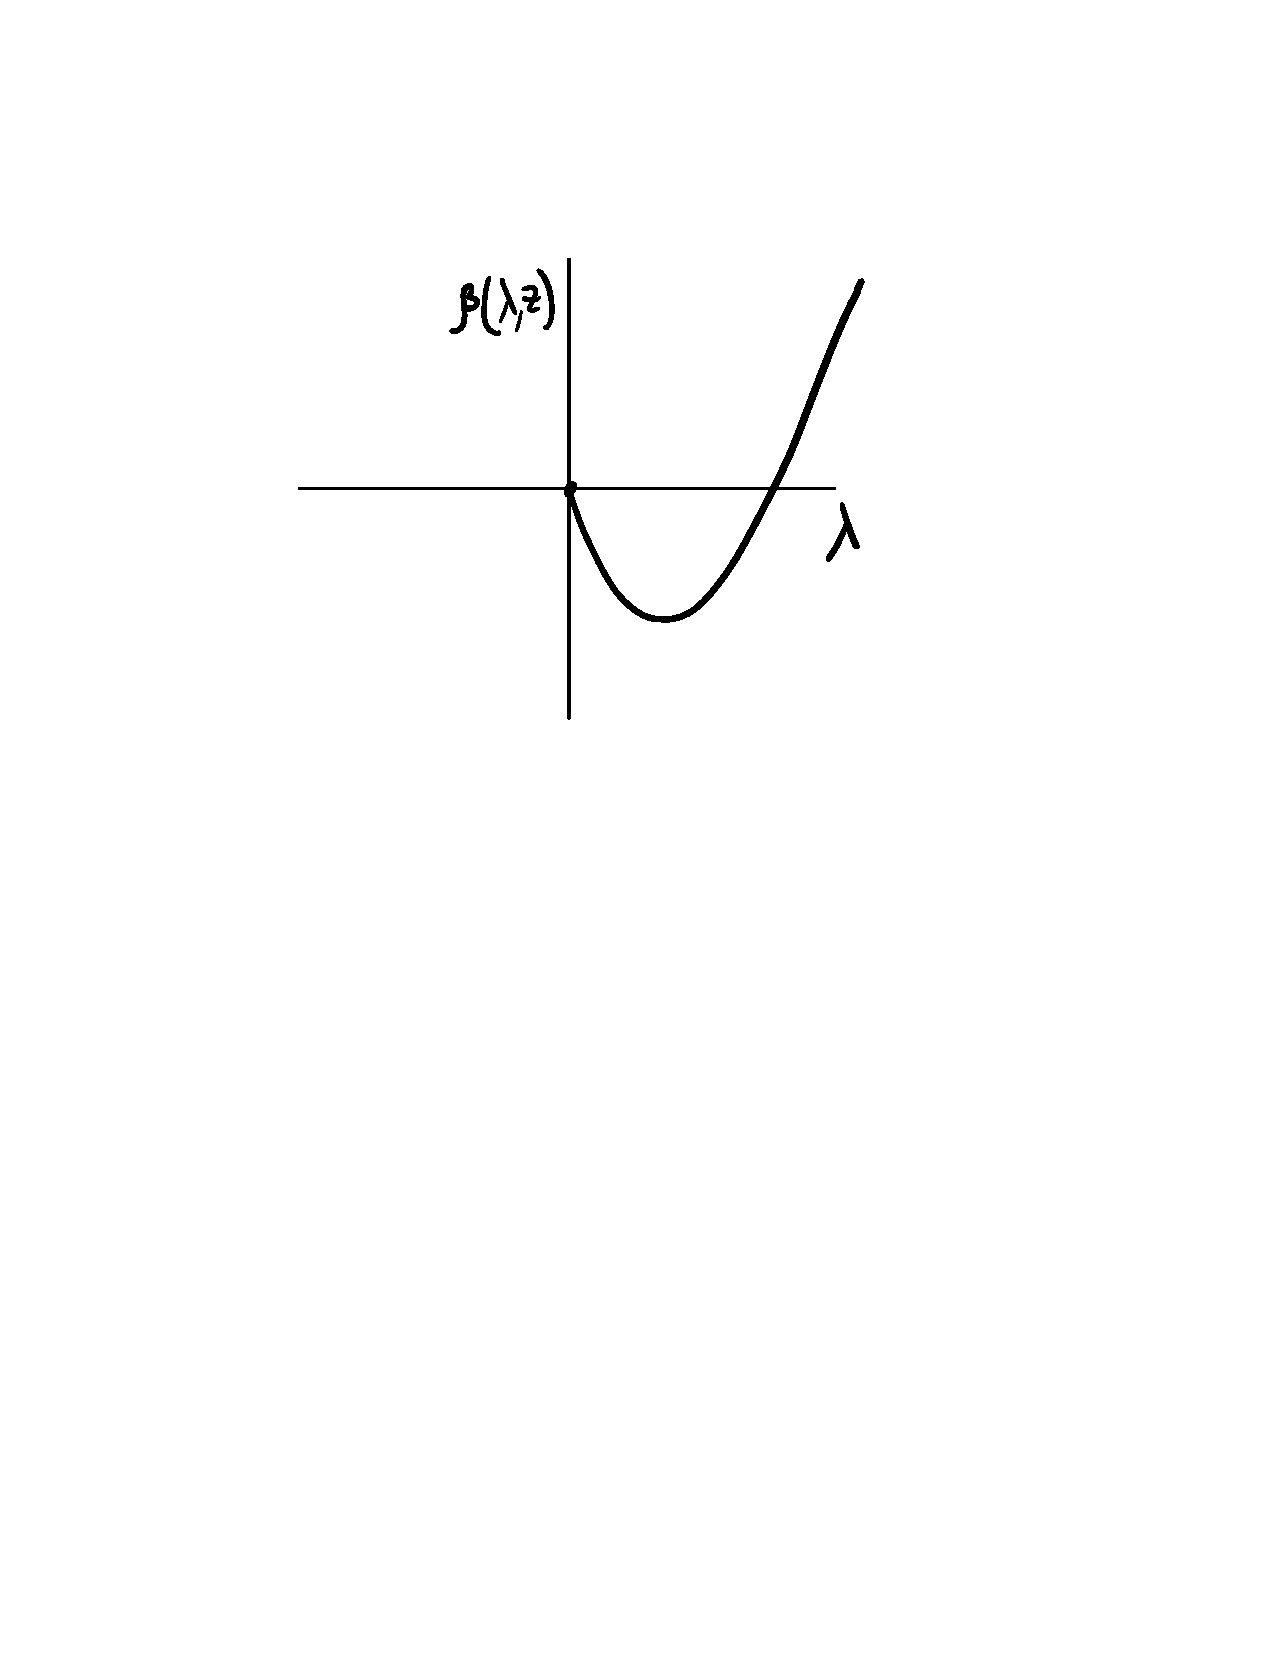
\includegraphics[scale=0.7]{Images/fig-betaplot1.pdf}
    \caption{Graph of $\beta$ function.}
    \label{fig-betaplot1}
\end{figure}

If the RHS is zero somehow, the flow stops. So, there are fixed points of the flow. If we start in the gap, we are trapped between two zeros in the $\beta$ function, and integrating more parts of the fields pushes us towards the right fixed point; $\lambda = \frac{128\pi^2}{3}\e$. So, we can integrate out into we flow to that point, and use this to compute something.

